\chapter{Исследовательская часть}

В данном разделе будут приведены примеры работы программы, и проведены замеры процессорного времени и предоставлена информация о технических характеристиках устройства.

\section{Технические характеристики}

Ниже представлены характеристики компьютера, на котором проводились замеры времени работы реализации алгоритмов:

\begin{itemize}
	\item операционная система Windows 10 Домашняя 21H2;
	\item оперативная память 12 Гб;
	\item процессор Intel(R) Core(TM) i7-9750H CPU @ 2.6ГГц.
\end{itemize}

Загруженность компонентов:

\begin{itemize}
	\item процессор --- 10\%;
	\item оперативная память --- 53\%
\end{itemize}

\clearpage

\section{Демонстрация работы программы}

На рисунке \ref{img:example} -- \ref{img:example3} приведены примеры работы программы.

\begin{figure}[h]
	\begin{center}
		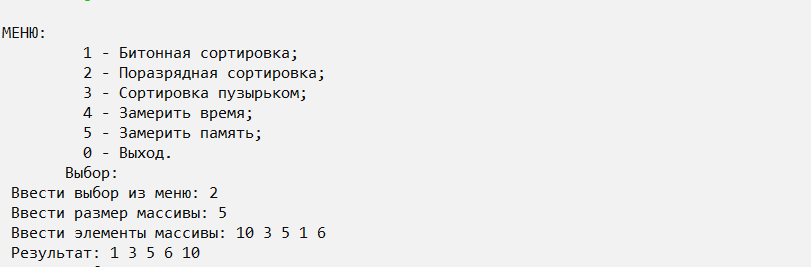
\includegraphics[scale=0.7]{img/example.png}
	\end{center}
	\captionsetup{justification=centering}
	\caption{Пример работы алгоритма битонной сортировки}
	\label{img:example}
\end{figure}


\begin{figure}[h]
	\begin{center}
		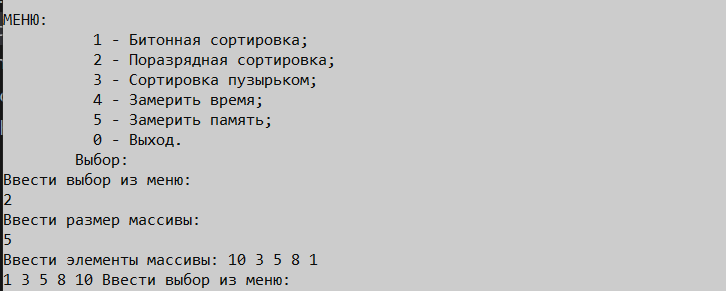
\includegraphics[scale=0.7]{img/example2.png}
	\end{center}
	\captionsetup{justification=centering}
	\caption{Пример работы алгоритма поразрядной сортировки}
	\label{img:example2}
\end{figure}
\clearpage

\begin{figure}[h]
	\begin{center}
		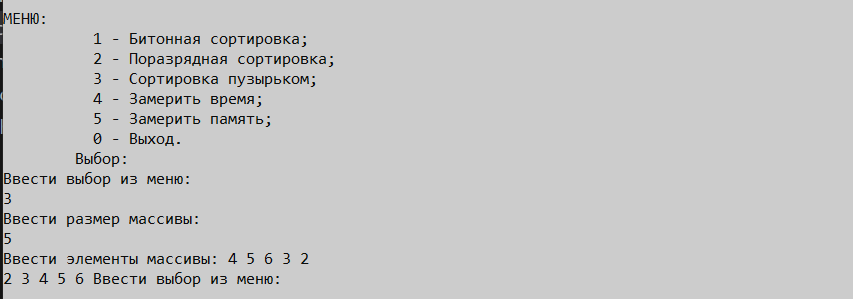
\includegraphics[scale=0.6]{img/example3.png}
	\end{center}
	\captionsetup{justification=centering}
	\caption{Пример работы алгоритма сортировки пузырьком}
	\label{img:example3}
\end{figure}

\section{Временные характеристики}

Функция clock() из библиотеки time.h языка программирования C возвращает процессорное время в секундах - значение типа clock\_t.

Для замера времени:
\begin{itemize}
	\item получить значение времени до начала выполнения алгоритма, затем после её окончания. Чтобы получить результат, необходимо вычесть из второго значения первое;
	\item первый шаг необходимо повторить iters раз (в программе iters равно 10), суммируя полученные значения, а затем усреднить результат.
\end{itemize}

Результаты эксперимента замеров по времени приведены в таблицах~\ref{tbl:random} -- ~\ref{tbl:des}.

В таблице~\ref{tbl:random} приведены результаты замеров по времени алгоритмов сортировок неотсортированных массивов, размером которых от 2 до 512. 
\begin{table}[h]
    \begin{center}
        \begin{threeparttable}
        \captionsetup{justification=raggedright,singlelinecheck=off}
        \caption{Результаты замеров времени (неотсортированный массив).}
        \label{tbl:random}
        \begin{tabular}{|c|c|c|c|}
        	\hline
        	& \multicolumn{3}{c|}{\bfseries Выходные данные по алгоритму, с} \\\cline{2-4}
        	Размер & Битонная & Поразрядная  & Пузырьком  
        	\csvreader{time_random.csv}{}
        	{\\\hline\csvcoli & \csvcolii & \csvcoliii & \csvcoliv} \\
        	\hline
        \end{tabular}
    \end{threeparttable}
\end{center}
\end{table}

На рисунке \ref{img:time_random} приведены графические результаты сравнения временных характеристик для неотсортированных массивов.

\begin{figure}[h]
	\begin{center}
		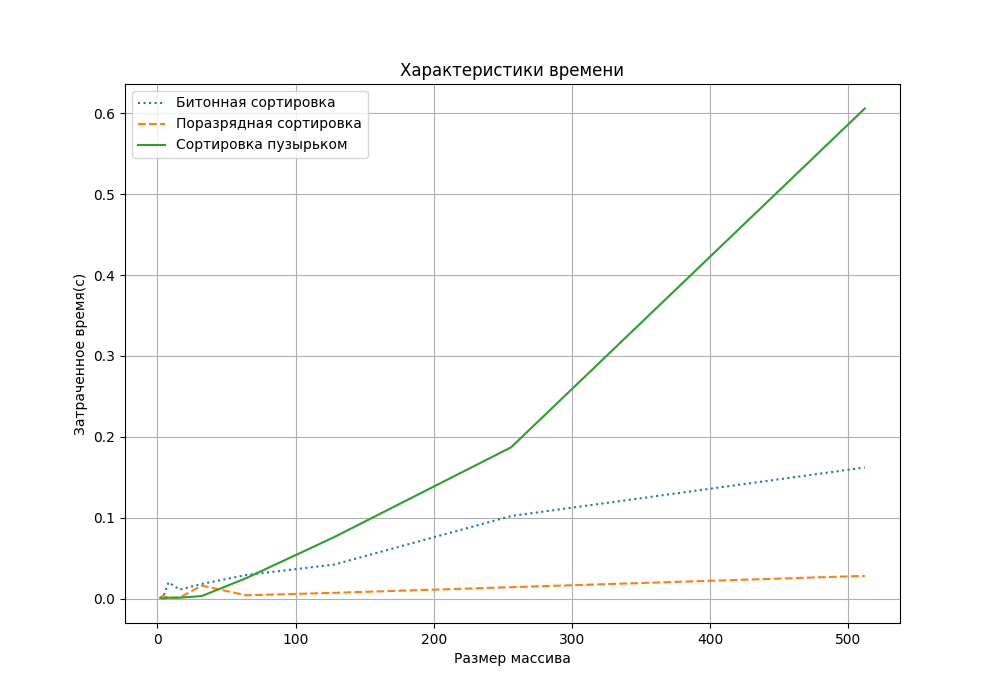
\includegraphics[scale=0.6]{img/time_random.png}
	\end{center}
	\captionsetup{justification=centering}
	\caption{Сравнение по времени алгоритмов сортировок неотсортированных массивов}
	\label{img:time_random}
\end{figure}
\clearpage
В таблице~\ref{tbl:ins} приведены результаты замеров по времени алгоритмов сортировок отсортированных массивов по возрастанию, размером которых от 2 до 512. 
\begin{table}[h]
	\begin{center}
		\begin{threeparttable}
			\captionsetup{justification=raggedright,singlelinecheck=off}
			\caption{Результаты замеров времени (неотсортированный массив по возрастанию).}
			\label{tbl:ins}
			\begin{tabular}{|c|c|c|c|}
				\hline
				& \multicolumn{3}{c|}{\bfseries Выходные данные по алгоритму, с} \\\cline{2-4}
				Размер & Битонная & Поразрядная  & Пузырьком  
				\csvreader{time_ins.csv}{}
				{\\\hline\csvcoli & \csvcolii & \csvcoliii & \csvcoliv} \\
				\hline
			\end{tabular}
		\end{threeparttable}
	\end{center}
\end{table}
\clearpage
На рисунке \ref{img:time_ins} приведены графические результаты сравнения временных характеристик для отсортированных массивов по возрастанию.

\begin{figure}[h]
	\begin{center}
		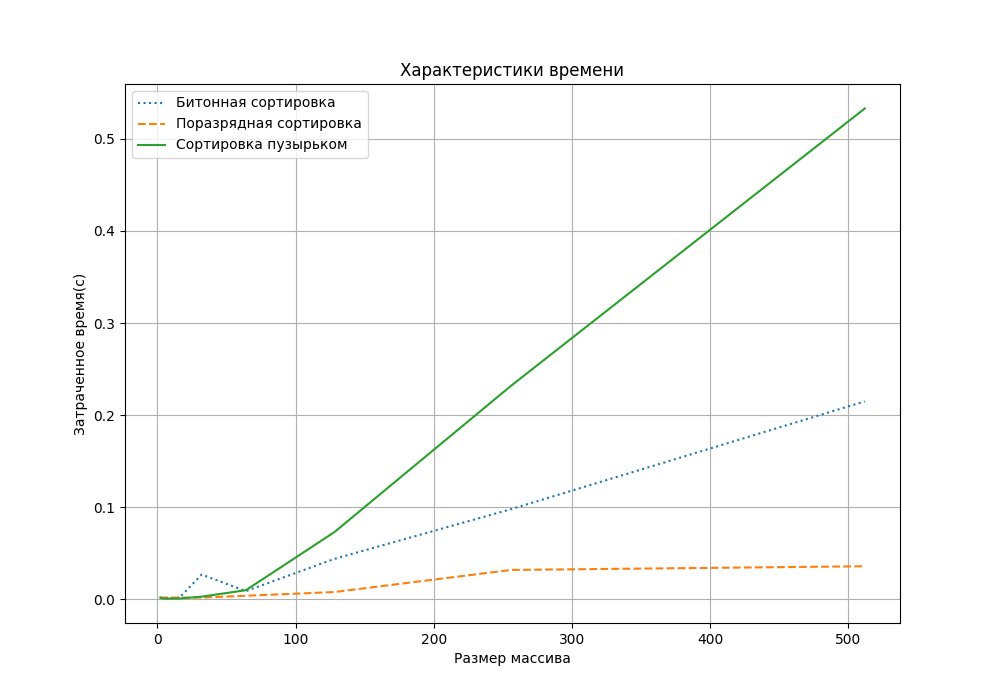
\includegraphics[scale=0.6]{img/time_ins.png}
	\end{center}
	\captionsetup{justification=centering}
	\caption{Сравнение по времени алгоритмов сортировок отсортированных массивов по возрастанию}
	\label{img:time_ins}
\end{figure}
\clearpage
В таблице~\ref{tbl:des} приведены результаты замеров по времени алгоритмов сортировок отсортированных массивов по убыванию, размером которых от 2 до 512. 
\begin{table}[h]
	\begin{center}
		\begin{threeparttable}
			\captionsetup{justification=raggedright,singlelinecheck=off}
			\caption{Результаты замеров времени (неотсортированный массив по убыванию).}
			\label{tbl:des}
			\begin{tabular}{|c|c|c|c|}
				\hline
				& \multicolumn{3}{c|}{\bfseries Выходные данные по алгоритму, с} \\\cline{2-4}
				Размер & Битонная & Поразрядная  & Пузырьком  
				\csvreader{time_des.csv}{}
				{\\\hline\csvcoli & \csvcolii & \csvcoliii & \csvcoliv} \\
				\hline
			\end{tabular}
		\end{threeparttable}
	\end{center}
\end{table}

На рисунке \ref{img:time_des} приведены графические результаты сравнения временных характеристик для отсортированных массивов по возрастанию.

\begin{figure}[h]
	\begin{center}
		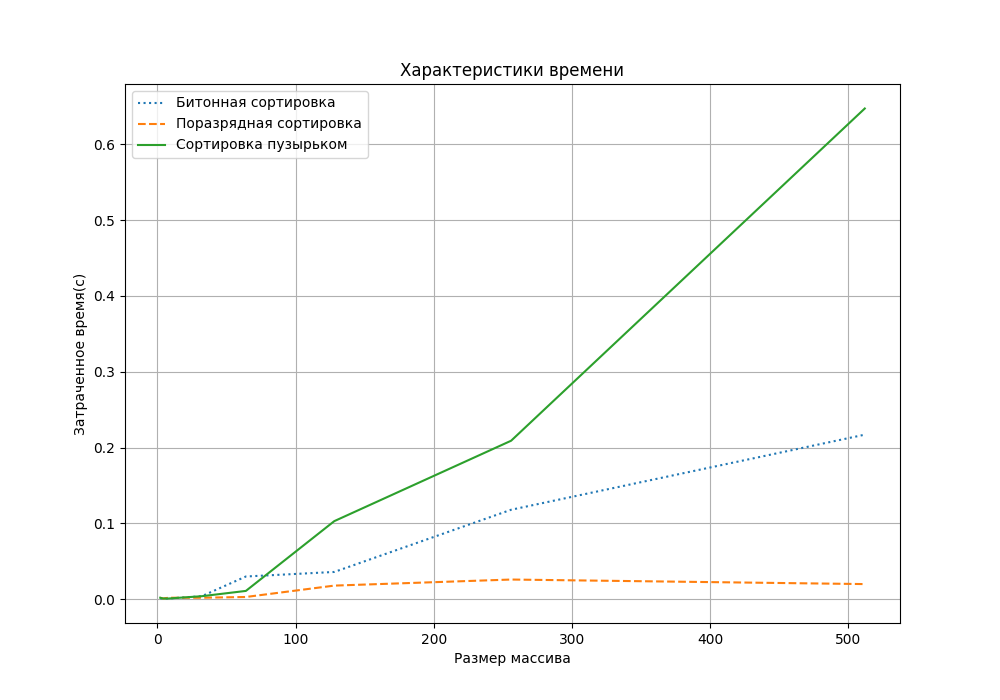
\includegraphics[scale=0.6]{img/time_des.png}
	\end{center}
	\captionsetup{justification=centering}
	\caption{Сравнение по времени алгоритмов сортировок отсортированных массивов по убыванию}
	\label{img:time_des}
\end{figure}
\clearpage

\section{Характеристики по памяти}

Пусть N — количество элементов массива, M — максимальное значение массива, тогда затраты памяти на рассматриваемые алгоритмы будут следующими.

Затраты по памяти для реализации алгоритма битонной сортировки:
\begin{itemize}
	\item массив: $N \cdot \text{sizeof}(\text{int})$;
	\item размер массива B: $\text{sizeof}(\text{int})$;
	\item дополнительные переменные (k, cnt, i, low): $4\cdot \text{sizeof}(\text{int})$;
\end{itemize}

Итого:
\begin{equation}
	\label{eq:bitonic}
	N \cdot \text{sizeof}(\text{int}) + \text{sizeof}(\text{int}) + 4\cdot \text{sizeof}(\text{int}) = (N + 5) \cdot \text{sizeof}(\text{int}) 
\end{equation}

Затраты по памяти для реализации алгоритма поразрядная сортировка:
\begin{itemize}
	\item массив: $N \cdot \text{sizeof}(\text{int})$;
	\item размер массива B: $\text{sizeof}(\text{int})$;
	\item дополнительные переменные: $8\cdot \text{sizeof}(\text{int})$;
	\item дополнительные массивы count, output: $(N + 10) \cdot\text{sizeof}(\text{int})$;
	\item адрес возврата.
\end{itemize}

Итого:
\begin{equation}
	\label{eq:wino_alg}
	N \cdot \text{sizeof}(\text{int}) + \text{sizeof}(\text{int}) + 8\cdot \text{sizeof}(\text{int}) + (N + 10) \cdot\text{sizeof}(\text{int}) = (2 \cdot N + 19) \cdot \text{sizeof}(\text{int}) 
\end{equation}

Затраты по памяти для реализации алгоритма сортировки пузырьком:
\begin{itemize}
	\item массив: $N \cdot \text{sizeof}(\text{int})$;
	\item размер массива B: $\text{sizeof}(\text{int})$;
	\item дополнительные переменные (i, j, c): $3\cdot \text{sizeof}(\text{int})$;
\end{itemize}

Итого:
\begin{equation}
	\label{eq:optimized_alg}
		N \cdot \text{sizeof}(\text{int}) + \text{sizeof}(\text{int}) + 3\cdot \text{sizeof}(\text{int}) = (N + 4) \cdot \text{sizeof}(\text{int}) 
\end{equation}

На рисунке \ref{img:mem} также приведены результаты замеров памяти. 

\begin{figure}[h]
	\begin{center}
		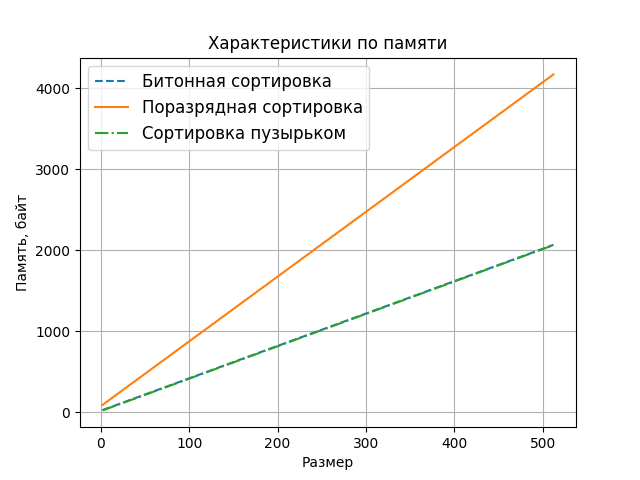
\includegraphics[scale=0.7]{img/mem.png}
	\end{center}
	\captionsetup{justification=centering}
	\caption{Сравнение по памяти алгоритмов сортировок}
	\label{img:mem}
\end{figure}
\section{Вывод}
В результате эксперимента было получено, что при размере массива больше 128, алгоритм сортировки пузырьком работает медленее алгоритма битонной сортировки в 1.8 раза и алгоритма поразрядной сортировки в 10.8 раза.
В случае, если массив уже отсортирован, время выполнения сортировки пузырьком в 1.2 раза убывается, так как не нужно выполнять обмен элементы.

Проведя анализ оценки затрат реализаций алгоритмов по памяти, можно сказать, что поразрядная сортировка больше затратны, так как для них использовать дополнительные массивы.
Затраты по памяти для алгоритма битонной сортировки и сортировки пузырьком не отличаются друг от друга.